\documentclass{beamer}

% This file is a solution template for:

% - Talk at a conference/colloquium.
% - Talk length is about 20min.
% - Style is ornate.



% Copyright 2004 by Till Tantau <tantau@users.sourceforge.net>.
%
% In principle, this file can be redistributed and/or modified under
% the terms of the GNU Public License, version 2.
%
% However, this file is supposed to be a template to be modified
% for your own needs. For this reason, if you use this file as a
% template and not specifically distribute it as part of a another
% package/program, I grant the extra permission to freely copy and
% modify this file as you see fit and even to delete this copyright
% notice. 


\mode<presentation>
{
  \usetheme{Madrid}
  % or ...

  \setbeamercovered{transparent}
  % or whatever (possibly just delete it)
}


\usepackage{listings}
\usepackage[english]{babel}

% or whatever

\usepackage[latin1]{inputenc}
% or whatever

\usepackage{times}
\usepackage[T1]{fontenc}
% Or whatever. Note that the encoding and the font should match. If T1
% does not look nice, try deleting the line with the fontenc.


%signals, used in Ingo's figures
\newcommand{\signal}[1]{$\overrightarrow{#1}$}

\graphicspath{{../report/figures/}{figures/}}

% grey for the listings


% settings for the listings
\lstset{language=Haskell,
  linewidth=.9\linewidth,
  stringstyle=\ttfamily,
  basicstyle=\scriptsize\ttfamily,
  frame=lines,
  frameround=ffff,
  backgroundcolor=\color[rgb]{.9,.9,1}}


\title%[Short Paper Title]  (optional, use only with long paper titles)
{ForSyDe's embedded compiler}

\subtitle{Third development stage results.}

\author[A.Acosta] % (optional, use only with lots of authors)
{Alfonso Acosta\\
\footnotesize \href{mailto:alfonso.acosta@gmail.com}{\nolinkurl{alfonso.acosta@gmail.com}}}

% - Give the names in the same order as the appear in the paper.
% - Use the \inst{?} command only if the authors have different
%   affiliation.

\institute[KTH] % (optional, but mostly needed)
{ICT/ECS\\Royal Institute of Technology, Stockholm}
% - Use the \inst command only if there are several affiliations.
% - Keep it simple, no one is interested in your street address.

\date%[CFP 2003] % (optional, should be abbreviation of conference name)
{August 19th, 2008}
% - Either use conference name or its abbreviation.
% - Not really informative to the audience, more for people (including
%   yourself) who are reading the slides online

\subject{Compilers}
% This is only inserted into the PDF information catalog. Can be left
% out. 



% If you have a file called "university-logo-filename.xxx", where xxx
% is a graphic format that can be processed by latex or pdflatex,
% resp., then you can add a logo as follows:

\pgfdeclareimage[height=0.5cm]{university-logo}{kth_cmyk}
\logo{\pgfuseimage{university-logo}}



% Delete this, if you do not want the table of contents to pop up at
% the beginning of each subsection:
\AtBeginSubsection[]
{
  \begin{frame}<beamer>
    \frametitle{Outline}
    \tableofcontents[currentsection,currentsubsection]
  \end{frame}
}

\AtBeginSection[]
{
  \begin{frame}<beamer>
    \frametitle{Outline}
    \tableofcontents[currentsection]
  \end{frame}
}


% If you wish to uncover everything in a step-wise fashion, uncomment
% the following command: 

\beamerdefaultoverlayspecification{<+->}


\begin{document}

\begin{frame}
  \titlepage
\end{frame}

\begin{frame}
  \frametitle{Outline}
  \tableofcontents[pausesections]
  % You might wish to add the option [pausesections]
\end{frame}


% Structuring a talk is a difficult task and the following structure
% may not be suitable. Here are some rules that apply for this
% solution: 

% - Exactly two or three sections (other than the summary).
% - At *most* three subsections per section.
% - Talk about 30s to 2min per frame. So there should be between about
%   15 and 30 frames, all told.

% - A conference audience is likely to know very little of what you
%   are going to talk about. So *simplify*!
% - In a 20min talk, getting the main ideas across is hard
%   enough. Leave out details, even if it means being less precise than
%   you think necessary.
% - If you omit details that are vital to the proof/implementation,
%   just say so once. Everybody will be happy with that.

\beamerdefaultoverlayspecification{}
\section{General Goal Review}
\begin{frame}
  \frametitle{General Goal Review}
  %\framesubtitle{Subtitles are optional.}
  % - A title should summarize the slide in an understandable fashion
  %   for anyone how does not follow everything on the slide itself.
  Plan set after last meeting (April 25th)
  \begin{itemize}
  \item<1-> July 1st.
    \begin{itemize}
    \item Automatic Test Suite with code
      coverage. \visible<2->{\pgfimage[height=10pt]{figures/tick}
        \alert{\small No CC due to TH.}}
    \item Stable VHDL Backend. \visible<2->{\pgfimage[height=10pt]{figures/tick}}
    \item Improve GraphML backend. \visible<2->{\pgfimage[height=10pt]{figures/tick}}
    \item Additional examples. \visible<2->{\pgfimage[height=10pt]{figures/tick}}
    \end{itemize}
  \item<3-> August 18th to August 24th: 3rd meeting at KTH.
    
  \item<4-> September 1st: Public release
    \begin{itemize}
      \item Full tutorial. \visible<5->{\pgfimage[height=10pt]{figures/tick}}
      \item Hacking Guide. \visible<5->{\pgfimage[height=10pt]{figures/cross}}
      \item Even more code examples. \visible<5->{\pgfimage[height=10pt]{figures/cross}}
      \item Implement Domain interfaces and other MoCs (Untimed,
        optionally CT), either
        .. \visible<5->{\pgfimage[height=10pt]{figures/tick} \alert{Option 2
          (Swallow-embedded \texttt{Signal})}}
        \begin{enumerate}
        \item porting them to the new deep-embedded \texttt{Signal} representation
        \item interfacing with the old swallow-embedded \texttt{Signal}.
        \end{enumerate}
    \end{itemize}
  \end{itemize}
\end{frame}

\section{Result details}

\subsection{Frontend}

\begin{frame}[fragile]
  \frametitle{Reminder: Design Flow Using Components (I)}
  %\framesubtitle{Components.}
  % - A title should summarize the slide in an understandable fashion
  %   for anyone how does not follow everything on the slide itself.
  \begin{itemize}
  \item
    Naive example of the design flow and API using components: Serial adder.
  \pgfimage[width=10cm]{figures/SeqAddFour}
  \end{itemize}
  
  
  \vspace{-0.7cm}
  \begin{overprint}
    \onslide<2>
   \begin{enumerate}[1)]
   \item Create a process function which adds one to its input 
    \begin{lstlisting}
  addOnef :: ProcFun (Int32 -> Int32)
  addOnef = $(newProcFun [d| addOnef :: Int32 -> Int32 
                             addOnef n = n + 1 |]
    \end{lstlisting}
    \end{enumerate}
   
   \onslide<3>
   \begin{enumerate}[2)]
   \item Create a system function corresponding to the unit adder
   \begin{lstlisting}
  addOneProc :: Signal Int32 -> Signal Int32
  addOneProc = mapSY "addOne" addOnef
   \end{lstlisting}
   \end{enumerate}
   
   \onslide<4>
   \begin{enumerate}[3)]
   \item Subsystem definition associated to the unit adder
   \begin{lstlisting}
 addOneSysDef :: SysDef (Signal Int32 -> Signal Int32)
 addOneSysDef = $(newSysDef 'addOneProc ["in1"] ["out1"])
   \end{lstlisting}
   \end{enumerate}


   \onslide<5>
   \begin{enumerate}[4)]
   \item Create the main system function
   \begin{lstlisting}
  addFour :: Signal Int32 -> Signal Int32
  addFour = $(instantiate "addOne3" 'addOneSysDef) .
            $(instantiate "addOne2" 'addOneSysDef) .
            $(instantiate "addOne1" 'addOneSysDef) .
            $(instantiate "addOne0" 'addOneSysDef)
   \end{lstlisting}
   \end{enumerate}

   \onslide<6>
   \begin{enumerate}[5)]
   \item Finally, build the main system definition
   \begin{lstlisting}
  addFourSys :: SysDef (Signal Int32 -> Signal Int32)
  addFourSys = $(newSysDef 'addFour ["in1"] ["out1"])
   \end{lstlisting}
   \end{enumerate}

\end{overprint}

\end{frame}

\begin{frame}
  \frametitle{Reminder: Design Flow Using Components (II)}
  %\framesubtitle{Design flow using components.}
  % - A title should summarize the slide in an understandable fashion
  %   for anyone how does not follow everything on the slide itself.
\vspace{-0.2cm}
\begin{center}
\pgfimage[height=8cm]{figures/compflow}
\end{center}

\end{frame}



\begin{frame}[fragile]
  \frametitle{Frontend Changes: Keep TH to a minimum (I)}
  %\framesubtitle{Components.}
  % - A title should summarize the slide in an understandable fashion
  %   for anyone how does not follow everything on the slide itself.
  \begin{itemize}
  \item<1-> The frontend functions \texttt{newSysDef},
    \texttt{instantiate} and \texttt{simulate} don't depend on
    Template Haskell anymore.

\begin{lstlisting}
newSysDef :: Name -> [PortId] -> [PortId] -> Q Exp
 -- sysfun -> [PortId] -> [PortId] -> SysDef (sysfun)
instantiate :: Name -> ProcId -> Q Exp -- SysDef a -> a
simulate :: Name -> Q Exp -- SysDef a -> listbased a 
\end{lstlisting}
\begin{lstlisting}
newSysDef :: (SysFun f) => f -> SysId -> 
                           [PortId] -> [PortId] ->
                           SysDef f
instantiate :: (SysFun f) => ProcId -> SysDef f -> f
simulate :: (SysFunToSimFun sysFun simFun) => 
            SysDef sysFun -> simFun
\end{lstlisting}

\item<2->     
  \begin{itemize}
  \item Saves the user from the inconvenient TH syntax.
  \item System patterns involving instantiate are now possible
  \item Does not suffer the type-inference problems of TH.
  \item Typing of frontend functions becomes helpful and intuitive.
  \item \alert{Drawback}: compile-time checks are lost (\texttt{newSysDefTH}).
  \end{itemize}
\end{itemize}
\end{frame}


\begin{frame}[fragile]
  \frametitle{Frontend Changes: Keep TH to a minimum (II)}
  %\framesubtitle{Components.}
  % - A title should summarize the slide in an understandable fashion
  %   for anyone how does not follow everything on the slide itself.
  \begin{itemize}
  \item<1-> System functions are variadic. 
    \begin{itemize}
    \item Is it possible to describe them with type classes
      (\texttt{SysFun} and \texttt{SysFunToSimFun})?
    \end{itemize}
  \item<2-> Yes! Solution inspired in \texttt{Text.Printf}.
  \item<3-> Sparing the class methods implementing the variadic ``magic''..
\begin{lstlisting}
class SysFun f 
instance SysFun ()
instance ProcType o => SysFun (Signal o)
instance (ProcType o1, ProcType o2) => SysFun (Signal o1, Signal o2)
... -- up to GHC's maximum: 62 elements
instance (ProcType i, SysFun f) => SysFun (Signal i -> f)
\end{lstlisting}
\begin{lstlisting}
class SysFun sysFun => SysFunToSimFun sysFun simFun -- no methods
 | sysFun -> simFun, simFun -> sysFun
instance SysFunToSimFun () ()
instance ProcType o => 
         SysFunToSimFun (Signal o) ([o])
... -- up to GHC's maximum: 62 elements
instance (ProcType a, SysFunToSimFun sysFun simFun) =>
         SysFunToSimFun (Signal a -> sysFun) ([a] -> simFun) 
\end{lstlisting}
\end{itemize}
\end{frame}

\begin{frame}[fragile]
  \frametitle{Frontend Changes:  ProcType (I)}
  %\framesubtitle{Components.}
  % - A title should summarize the slide in an understandable fashion
  %   for anyone how does not follow everything on the slide itself.
  \begin{itemize}
  \item<1-> The \texttt{ProcType} typeclass denotes which values can be
    carried by signals.
  \item<2-> The restriction is guaranteed by construction, e.g.
\begin{lstlisting}
constSY :: (ProcType a) => ProcId -> a -> Signal a
\end{lstlisting}    
  \item<3-> Definition of \texttt{ProcType}
\begin{lstlisting}
class ({Typeable a,} Data a, Lift a) => ProcType a where
\end{lstlisting}
    \begin{itemize}
      \item \texttt{Typeable}: Type information, used to support
        dynamic typing. Needed for type mapping (VHDL backend)
      \item \texttt{Data}: Structural information about a type. 
        \alert{Support for enumerated types in translation-backends!}
      \item \texttt{Lift}: Liftable values. Values of which a TH
        Expression-AST can be obtained. Needed for the translation of
        constant values passed to process constructors.
    \end{itemize}
  \end{itemize}
\end{frame}

\begin{frame}[fragile]
  \frametitle{Frontend Changes:  ProcType (II)}
  %\framesubtitle{Components.}
  % - A title should summarize the slide in an understandable fashion
  %   for anyone how does not follow everything on the slide itself.
  \begin{itemize}
  \item<1-> \texttt{ProcType} instances omitting its methods
\begin{lstlisting}
instance (Data a, Lift a) => ProcType a
instance (ProcType a, Nat s) => FSVec s a
instance ProcType a => ProcType (AbstExt a)
instance (ProcType i1, ProcType i2) => ProcType (i1, i2)
... -- up to GHC's maximum: 62 elements
instance ProcType a => ProcType (AbstExt a)
\end{lstlisting}
  \item<2-> Overlapped-instances are required to obtain the
    type-definition of values nested in structures.
  \item<3-> The \texttt{ProcType} instantiation hassle is almost negligible.
    \begin{overprint}
      \onslide<3>
\begin{lstlisting}
data MyColor = Red | Green | Blue
 deriving (Data, Typeable)

$(deriveLift1 ''MyColor)
\end{lstlisting}
      \onslide<4>
\begin{lstlisting}
data MyColor = Red | Green | Blue
 deriving (Data, Typeable)

-- new "Data a => Lift a" overlapping instance
\end{lstlisting} 
\end{overprint}     
    
  \end{itemize}
\end{frame}

\subsection{GraphML backend}

\beamerdefaultoverlayspecification{}
\begin{frame}
  \frametitle{GraphML backend (I)}
  %\framesubtitle{Components.}
  % - A title should summarize the slide in an understandable fashion
  %   for anyone how does not follow everything on the slide itself.
  \begin{itemize}
  \item Backend option to add yFiles-specific graphical markup
    \begin{itemize}
    \item Node colors, shape and size (base on source/target signals).
    \item Edge arrows, and location (making sharing of source signals possible).
    \end{itemize}

    \begin{tabular}{c}
      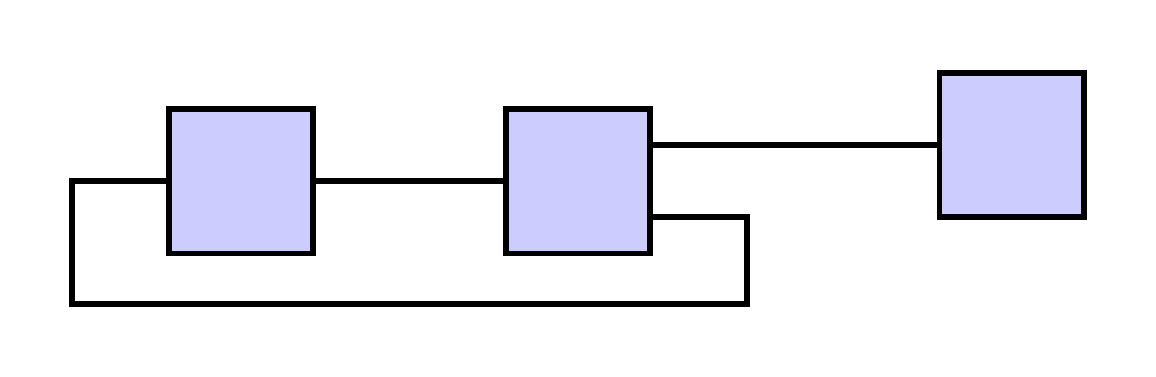
\includegraphics[height=2.5cm]{figures/counter}\\
      \hline
      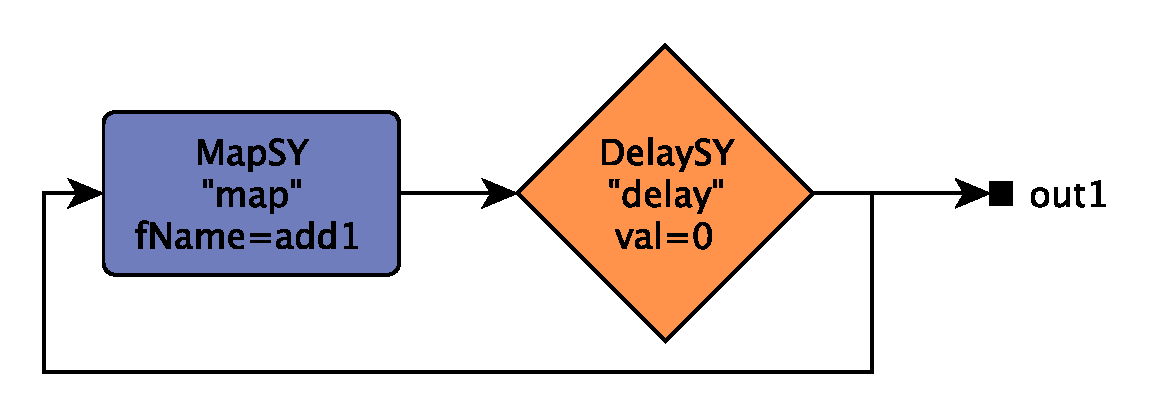
\includegraphics[height=2.5cm]{figures/counter_yFiles}\\
    \end{tabular}
  \end{itemize}
  
\end{frame}

\beamerdefaultoverlayspecification{<+->}
\begin{frame}
  \frametitle{GraphML backend (II)}
  %\framesubtitle{Components.}
  % - A title should summarize the slide in an understandable fashion
  %   for anyone how does not follow everything on the slide itself.
  \begin{itemize}
  \item Neither GraphML nor yFiles-GraphML suit all our needs
    \begin{itemize}
    \item yFiles doesn't respect GraphML ports (source signal
      sharing)
      \begin{itemize}
      \item solution: precalculate the location of
        edge ends $+$ routing port constraints (cannot be saved).
      \end{itemize}
    \item yEd wipes out external \texttt{<data>} tags.
      \begin{itemize}
      \item Once a GraphML file is opened and saved by yEd, ForSyDe's metadata
        (e.g. \texttt{ProcFun}s) is lost.
      \end{itemize}
    \item GraphML nor yFiles-GraphML support subgraph sharing
      (components)
      \begin{itemize}
      \item solution: use external \texttt{<data>} tags indicating
        parent systems in instance nodes.
      \item yEd is unaware of that information $\rightarrow$
        no hierarchical browsing.
      \end{itemize}      
    \end{itemize}
  \end{itemize}
  
\end{frame}


\subsection{VHDL backend}

\begin{frame}[fragile]
  \frametitle{VHDL backend}
  %\framesubtitle{Components.}
  % - A title should summarize the slide in an understandable fashion
  %   for anyone how does not follow everything on the slide itself.
  \begin{itemize}
  \item<1-> Pattern matching support in \texttt{ProcFuns}s, e.g.
\begin{lstlisting}
fstPF = $(newProcFun [d| fstPF (a,_) = a |])
\end{lstlisting}
  \item<2-> User-defined enumerated types (Algebraic types with
    zero-arity constructors) can now be mapped to VHDL.
\begin{lstlisting}
data Direction = Up | Down | Left | Right | Unknown
 deriving (Data, Typeable, Show, Eq)
buttonEncoder :: Signal (FSVec D4 Bit) -> Signal Direction
\end{lstlisting}    
    
  \item<3-> Support for 3rd party EDA tools
    \begin{itemize}
      \item<3-> Quartus II. The resulting VHDL model can me
        automatically analyzed (\texttt{analyzeQuartus} VHDL-Backend flag).
        \begin{itemize}
        \item<3-> The resulting project can be reused.
        \end{itemize}
      \item<4-> Modelsim. The VHDL model can be compiled and
        simulated.
        \begin{itemize}
          \item<5-> Compilation (\texttt{compileModelsim} VHDL-backend flag).
          \item<6-> Simulation, new function
\begin{lstlisting}
writeAndModelsimVHDL :: (SysFunToIOSimFun sysF simF) =>
                        Maybe Int -> SysDef sysF -> simF
\end{lstlisting}            
          \end{itemize}
        \item<7-> Especially useful for testing (dozens of bugs detected
          and fixed)
    \end{itemize}
  \end{itemize}
  
\end{frame}

\subsection{Installation/Testing}

\begin{frame}
  \frametitle{Installation/Testing}
  %\framesubtitle{Components.}
  % - A title should summarize the slide in an understandable fashion
  %   for anyone how does not follow everything on the slide itself.
  \begin{itemize}
  \item New test framework/suite based on HUnit.
  \item Two ways to run it
    \begin{enumerate}
    \item Cabal: \texttt{./Setup.hs test}
    \item Darcs repository, candidate patches are now automatically
      verified before pushed.
      \begin{enumerate}
      \item Only patches affecting the source tree are verified.
      \item The project is tested to compile and is installed inplace.
      \item The test suite is run.
      \end{enumerate}
    \end{enumerate}
  \item Unfortunately, due to ForSyDe's TH dependency, Code Coverage is not
    yet working (fixed for GHC 6.10).
  \item Test suite needs to be extended.
    \begin{itemize}
    \item Currently: verification of systems under
      \texttt{examples/} (simulation vs VHDL simulation)
    \item Future: erroneous tests, XML-Schema verification of
      GraphML backend, regresion tests ...
    \end{itemize}
  \item Installation change: ForSyDe's VHDL is now precompiled with Modelsim at
    installation-time.
  \end{itemize}
    
\end{frame}

\subsection{Integration of shallow-embedded MoCs}

\begin{frame}
  \frametitle{Integration of shallow-embedded MoCs}
  %\framesubtitle{Components.}
  % - A title should summarize the slide in an understandable fashion
  %   for anyone how does not follow everything on the slide itself.
  \begin{itemize}
  \item Merged the shallow-embedded implementation of ForSyDe under
    \texttt{ForSyDe.Shallow}.
  \item Possible to include deep-embedded signals in swallow-embedded
    systems using \texttt{simulate} (e.g. \texttt{DeepShallow.hs})
  \item GHC Warning,s mainly due to double exports: we need to fix this.
  \item Everyone should move to the new tree.
    \begin{itemize}
    \item Repository, Testing framework and Cabal packaging can be
      reused.
    \item The change only affects import declarations of existing code.
    \end{itemize}
  \end{itemize}
  
\end{frame}

\subsection{Documentation}

\begin{frame}
  \frametitle{Documentation}
  %\framesubtitle{Components.}
  % - A title should summarize the slide in an understandable fashion
  %   for anyone how does not follow everything on the slide itself.
  \begin{itemize}
  \item Tutorial
    \begin{itemize}
      \item Docbook format
    \end{itemize}
  \item Web page
  \begin{itemize}
    \item Add it to the repository.
    \item The \texttt{imit.kth.se} domain is outdated
    \item Use the new address
      \url{http://www.ict.kth.se/org/ict/ecs/sam/projects/forsyde/www/}
      and redirect \url{http://www.imit.kth.se/info/FOFU/ForSyDe/}
  \end{itemize}
  \item Next: Hacking guide.
  \end{itemize}
  
\end{frame}

\section{Finally: public release}

\begin{frame}
  \frametitle{Finally: public release}
  %\framesubtitle{Design flow using components.}
  % - A title should summarize the slide in an understandable fashion
 \begin{itemize}
 \item Version number: 0.1? 3.0?
 \item Contact email?
   \begin{itemize}
   \item Ideal solution: mailing list.
   \item Problem: \texttt{ecs\_forsyde\_development@ict.kth.se} is not
     publicly accesible outside KTH.
   \end{itemize}

 \item Shallow-embedded version can be made fully public?
 \item Should we make the Darcs repository public?
   \begin{itemize}
   \item It would require restructuring \texttt{doc/}.
   \item More traditional approach? (only punctual public releases).
   \end{itemize}
 \item Release note
   \begin{itemize}
     \item Points to emphasize?
     \item ForSyDe's teaser for the Haskell community: needs to be
       carefully reviewed.
     \end{itemize}
 \end{itemize}
\end{frame}


\section{What's next?}

\begin{frame}
  \frametitle{What's next?}
  %\framesubtitle{Design flow using components.}
  % - A title should summarize the slide in an understandable fashion
 \begin{itemize}
 \item What should be done now? 
 \item Get ready for the release.
   \begin{itemize}
     \item Release Note
     \item Code packaging and upload to HackageDB.
     \item Webpage update.
     \item Cleanup of compilation warnings.
   \end{itemize}
 \item Code cleanup (hopefully after some feedback).
 \item Hacking guide.
 \item Fix as many tracker issues as possible.
 \item More Examples? More Tests?
 \end{itemize}
\end{frame}

\end{document}


